\documentclass[11pt]{article}
\usepackage[top=1in, bottom=1in, right=1in, left=1in]{geometry} % margins
\usepackage[dvipsnames]{xcolor}
\usepackage{setspace}
\usepackage{booktabs}
\usepackage[toc]{appendix} % appendix part of table of contents
\usepackage{titlesec}
\usepackage{float} % position tables exactly where I want them
\usepackage{amsmath}
\usepackage{graphicx}
\usepackage{dcolumn}
\usepackage{changepage}
\usepackage{fixltx2e}
\usepackage{setspace}
\usepackage{url} % web links
\usepackage{listings}
\usepackage{rotating}
\usepackage[final]{changes} % track changes
\usepackage{bbding}
\usepackage{paralist} % for \compactitem
\usepackage{array}
\usepackage{titling} % to remove space between title and date in \maketitle
\usepackage{soul} % to highlight text with \hl (also wraps the text) -- if including a link, wrap link in \hbox{}
\usepackage{hyperref} % for links
\hypersetup{
    colorlinks = true,
    allcolors = blue
} % activates blue color for all links
\colorlet{Changes@Color}{red}
\errorcontextlines 10000
\newcolumntype{.}{D{.}{.}{-1}}
\newcolumntype{d}[1]{D{.}{.}{#1}}
\lstset{
basicstyle=\small\ttfamily,
columns=flexible,
breaklines=true
}
\usepackage{apacite}
\newcommand{\bibtex}{\textsc{Bib\TeX}}
\renewcommand\appendixname{Appendix}
\renewcommand\appendixpagename{Appendix}
\renewcommand\appendixtocname{Appendix}
\renewcommand\maketitlehookc{\vspace{-8ex}} % moves date up in \maketitle
\newlength{\mylen} % next 4 lines make that stupid bullet sign smaller and raise it to the same vertical height as the normal \bullet
\setbox1=\hbox{$\bullet$}\setbox2=\hbox{\tiny$\bullet$}
\setlength{\mylen}{\dimexpr0.5\ht1-0.5\ht2}
\renewcommand\labelitemi{\raisebox{\mylen}{\tiny$\bullet$}} 
\setlength{\droptitle}{-5em} % moves title up in \maketitle
\setlength\parindent{1cm}
\setremarkmarkup{(#2)}
\titleformat*{\section}{\normalsize\bfseries} % makes section titles a bit smaller but still bold
\titleformat*{\subsection}{\normalsize\itshape} % makes subsection titles a bit smaller but still bold
\titlespacing*{\section}{0pt}{0.4cm}{0cm} % reduces space before and deletes space after section title
\titlespacing*{\subsection}{0pt}{0.4cm}{0cm} % reduces space before and deletes space after subsection title
\graphicspath{ {figures/} } % loads figures from the "figures" folder (for aesthetics)
\bibliographystyle{apacite}
\newenvironment{coi}{\compactitem}{\endcompactitem} % renaming so I can type \begin{coi} instead of \begin{compactitem}
\pagenumbering{gobble} % to suppress page numbers
\usepackage{helvet} % next two lines use Arial font
\renewcommand{\familydefault}{\sfdefault}
% timeline:
\usepackage[utf8]{inputenc}
\usepackage[TS1,T1]{fontenc}
\usepackage{fourier, heuristica}
\usepackage{array, booktabs}
\usepackage{graphicx}
\usepackage{colortbl}
\usepackage{caption}
\DeclareCaptionFont{blue}{\color{NavyBlue}}
\newcommand{\foo}{\color{NavyBlue}\makebox[0pt]{\textbullet}\hskip-0.5pt\vrule width 1pt\hspace{\labelsep}}

\title{\textbf{\large{\textcolor{NavyBlue}{BRIEF BUDGET JUSTIFICATION}\\DOCTORAL STUDENT RESEARCH\\\vspace{-0.2cm}SCHOLARSHIP}}}

\date{}

\begin{document}

\maketitle

\vspace{-1.6cm}

\singlespacing


\noindent I am applying for this scholarship to raise the funds to cover the costs of pre-testing the survey questionnaire and fielding the survey twice online on MTurk. Under the definition of the Itemized Budget Form, these costs fall under the item heading ``Supplies and Materials". They amount to a total of \$4,830 and are itemized below. Two screenshots show the origin of the budget calculations.

\vspace{0.3cm}

\begin{table}[H]
\renewcommand\arraystretch{1.4}\arrayrulecolor{NavyBlue}
\captionsetup{singlelinecheck=false, font=blue, labelfont=sc, labelsep=quad}
\caption*{Requested Funds for Supplies and Materials: Data Sets}\vskip -1.5ex
\begin{tabular}{@{\,}r <{\hskip 2pt} !{\foo} >{\raggedright\arraybackslash}p{11cm}}
\toprule
\addlinespace[1.5ex]
\$350 & \textbf{Pre-testing the survey questionnaire online on MTurk} \hspace{1.5cm} 500 respondents \hspace{7cm} Compensation per respondent: \$0.50 \hspace{7cm} Amazon commission per respondent: \$0.20 \\
\$2,240 & \textbf{Fielding the survey with flip-a-coin randomization on MTurk} \hspace{1.5cm} 1,600 respondents \hspace{7cm} Compensation per respondent: \$1.00 \hspace{7cm} Amazon commission per respondent: \$0.40\\
\$2,240 & \textbf{Fielding the survey with sequential blocking on MTurk} \hspace{1.5cm} 1,600 respondents \hspace{7cm} Compensation per respondent: \$1.00 \hspace{7cm} Amazon commission per respondent: \$0.40\\
\end{tabular}
\end{table}


\begin{figure}[H]
  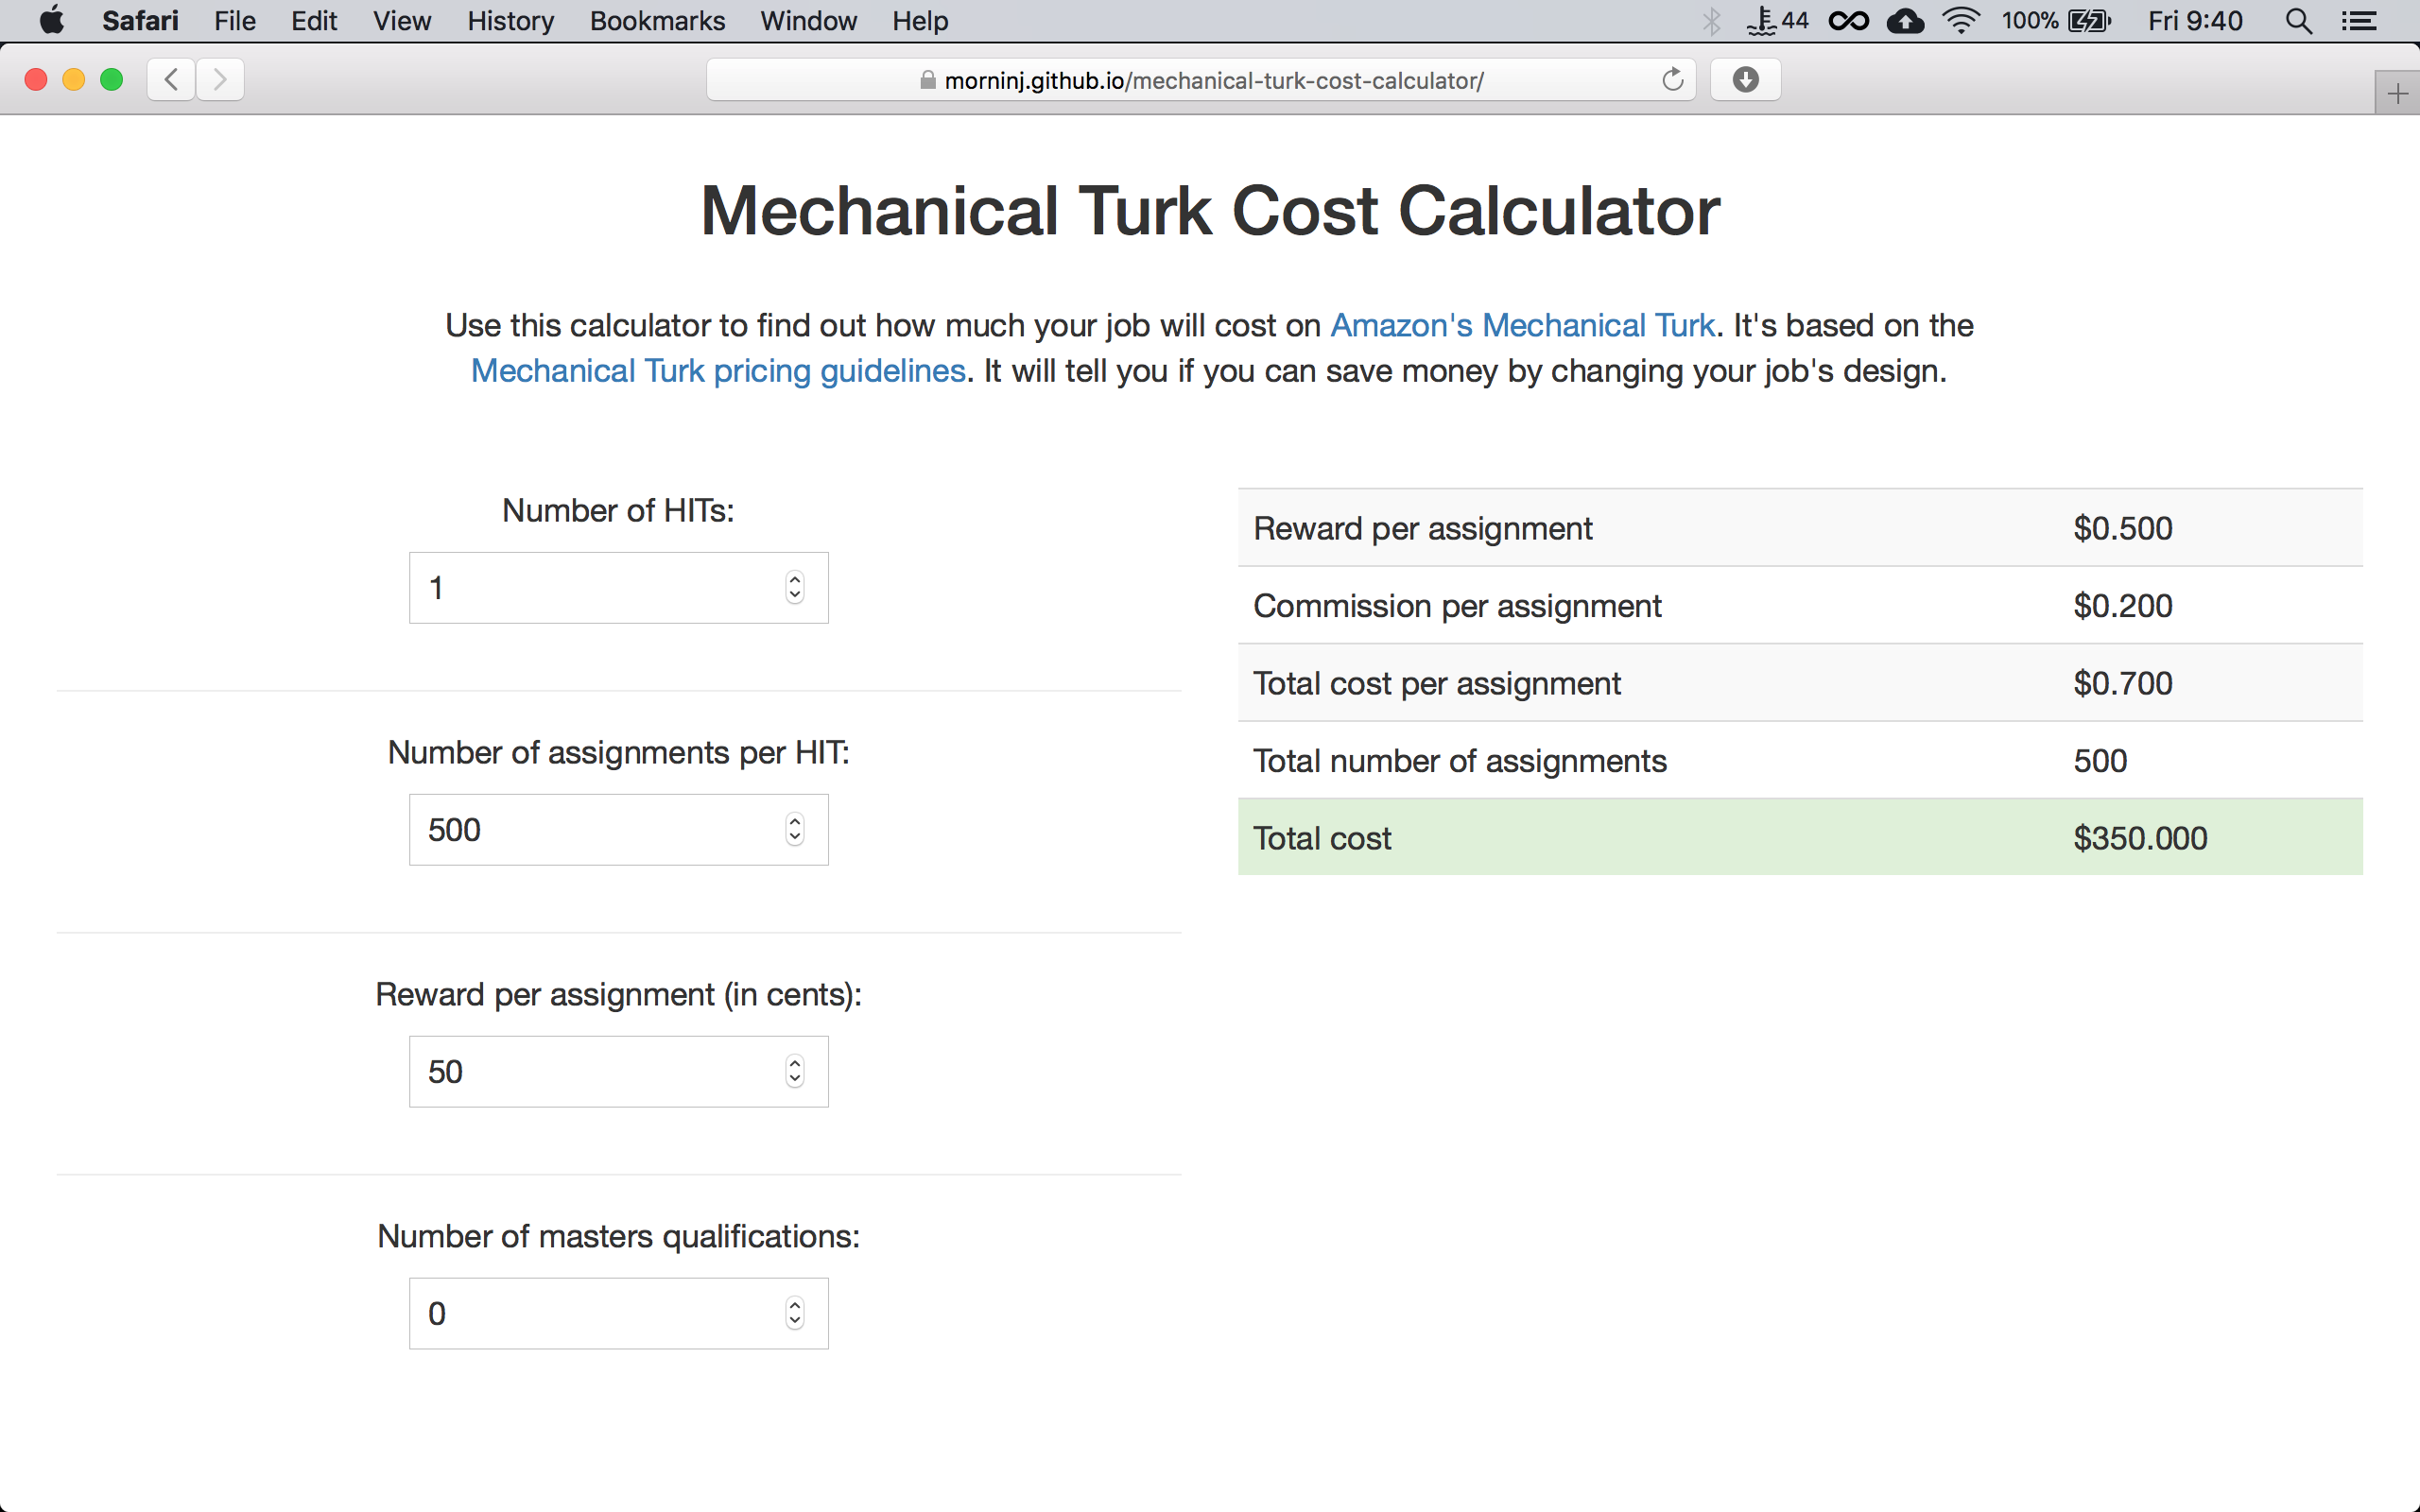
\includegraphics[width=\textwidth,height=.4\textheight,keepaspectratio]{survey_testing_costs.png}
\end{figure}

\begin{figure}[H]
  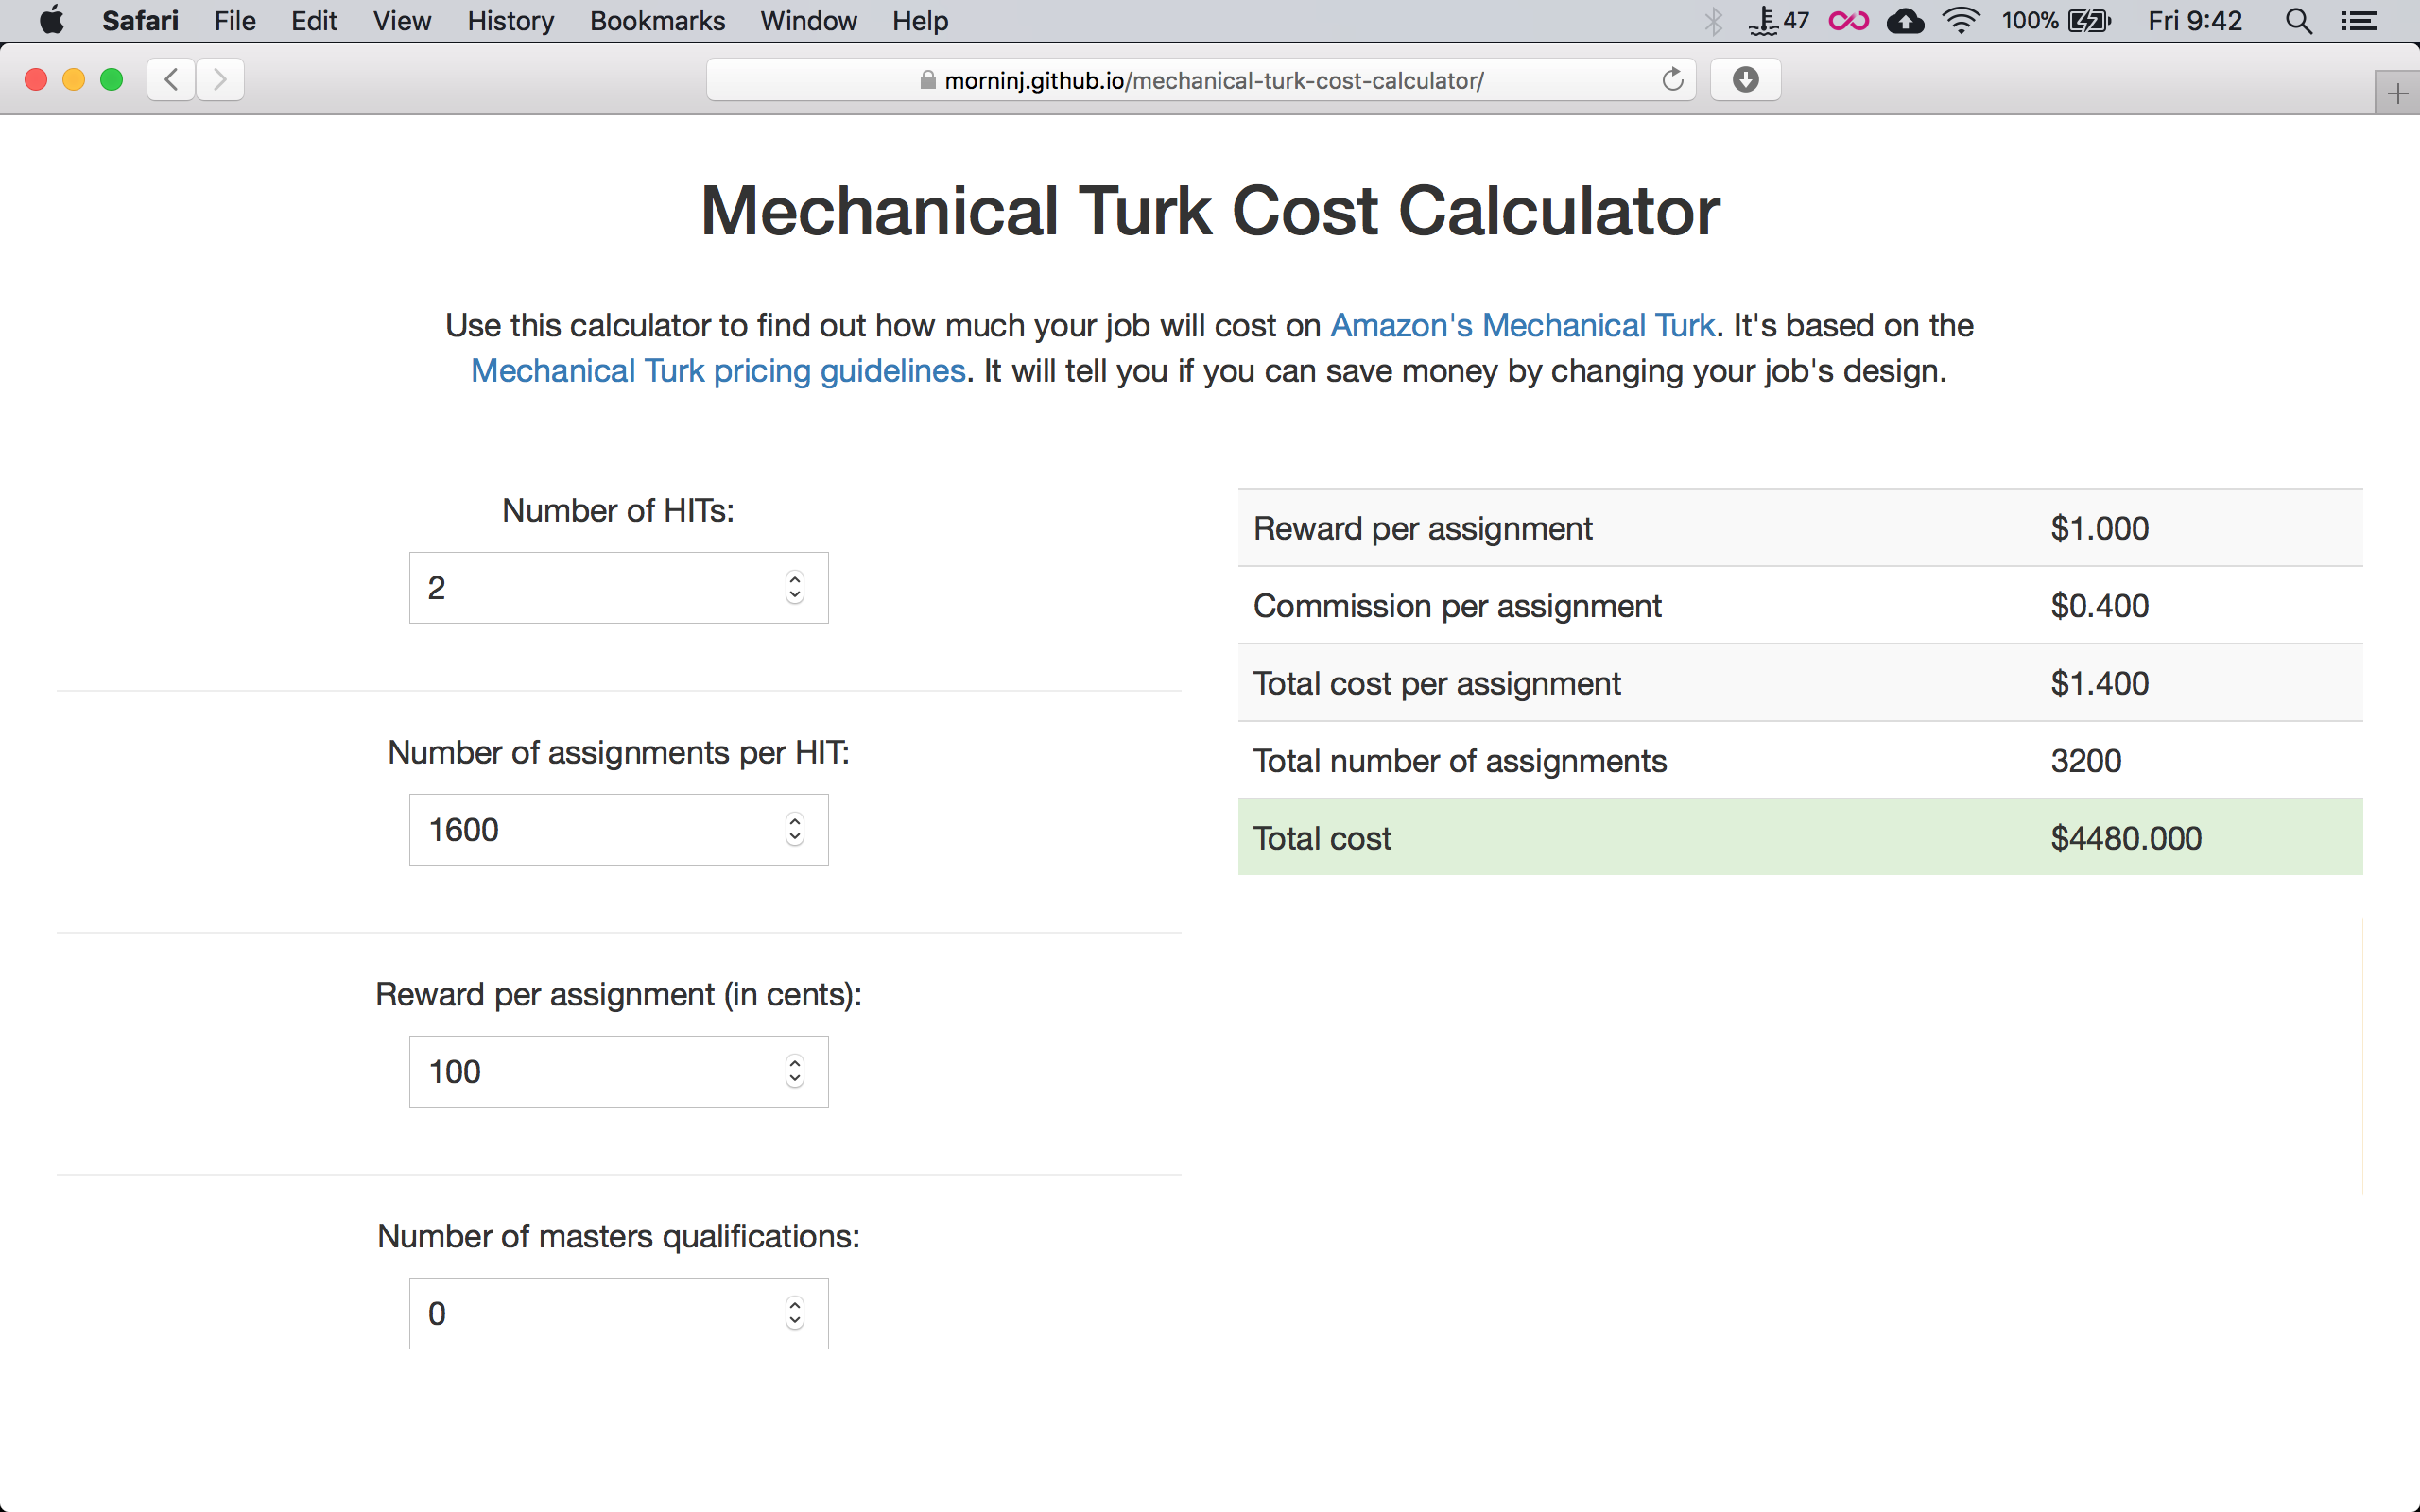
\includegraphics[width=\textwidth,height=.4\textheight,keepaspectratio]{survey_fielding_costs.png}
\end{figure}



% Jeff: Add screenshots of the MTurk cost calculator to this. Also reduce both n to 1,600





\end{document}


